% !TEX TS-program = pdflatex
% !TEX encoding = UTF-8 Unicode

% This is a simple template for a LaTeX document using the "article" class.
% See "book", "report", "letter" for other types of document.

% use larger type; default would be 10pt
\documentclass[11pt]{scrartcl}

% set input encoding (not needed with XeLaTeX)
\usepackage[utf8]{inputenc}
\usepackage[title,titletoc,header]{appendix}
\usepackage{multicol}
% \usepackage{titling}
\usepackage{longtable}

\usepackage{amsmath}
\usepackage{hyperref}

\usepackage{todonotes}
% \usepackage[disable]{todonotes}
\presetkeys{todonotes}{inline}{}

\usepackage{natbib}
% To cite, use \citet{} in text citation, or \citep{} (in parentheses).

%%% PAGE DIMENSIONS
\usepackage[a4paper]{geometry} % to change the page dimensions
% \geometry{a4paper, margin=1.3in} % or letterpaper (US) or a5paper or....
% \geometry{margin=2in} % for example, change the margins to 2 inches all round
% \geometry{landscape} % set up the page for landscape
%   read geometry.pdf for detailed page layout information

\usepackage{graphicx}               % support the \includegraphics command and options

% \usepackage[parfill]{parskip} % Activate to begin paragraphs with an empty line rather than an indent

%%% PACKAGES
\usepackage{booktabs}               % for much better looking tables
\usepackage{tabularx}
\renewcommand{\arraystretch}{1.5}
\usepackage{array}                  % for better arrays (eg matrices) in maths
\usepackage{paralist}               % very flexible & customisable lists (eg. enumerate/itemize, etc.)
\usepackage{verbatim}               % adds environment for commenting out blocks of text & for better verbatim
\usepackage{subfig}                 % make it possible to include more than one captioned figure/table in a single float
\usepackage{float}                  % allow floating for figures

\usepackage{pgfgantt}               % gantt charts
% \usepackage[export]{adjustbox}[2011/08/13] % For centering wide figures

%%% PARAGRAPHING & INDENTATION
\setlength{\parindent}{0pt}
\setlength{\parskip}{2ex plus 0.5ex minus 0.3ex}

%%% HEADERS & FOOTERS
\usepackage{fancyhdr}               % This should be set AFTER setting up the page geometry
\pagestyle{fancy}                   % options: empty , plain , fancy
\renewcommand{\headrulewidth}{0pt}  % customise the layout...
\lhead{}\chead{}\rhead{}
\lfoot{}\cfoot{\thepage}\rfoot{}

%%% SECTION TITLE APPEARANCE
\usepackage{sectsty}
\allsectionsfont{\sffamily\mdseries\upshape} % (See the fntguide.pdf for font help)
% (This matches ConTeXt defaults)

%%% ABSTRACT APPEARANCE
\usepackage{abstract}
\renewcommand{\absnamepos}{flushleft}
\setlength{\absleftindent}{0pt}
\setlength{\absrightindent}{0pt}

%%% TABLE OF CONTENTS APPEARANCE
 % Put the bibliography in the ToC
\usepackage[nottoc,notlof,notlot]{tocbibind}
 % Alter the style of the Table of Contents
\usepackage[titles,subfigure]{tocloft}
\renewcommand{\cftsecfont}{\rmfamily\mdseries\upshape}
 % No bold!
\renewcommand{\cftsecpagefont}{\rmfamily\mdseries\upshape}

%%% REFERENCES APPEARANCE
\renewcommand{\bibname}{References}

\newcommand{\code}[1]{{\texttt{#1}}}
\newcommand{\libraryname}[1]{{\texttt{#1}}}
\newcommand{\codefile}[1]{{\textit{#1}}}
\newcommand{\program}[1]{\code{#1}}
\newcommand{\taskname}[1]{{\textit{#1}}}
\newcommand{\mytilda}{\raise.17ex\hbox{$\scriptstyle\mathtt{\sim}$}}

\title{Sphere Detection using Boosted Classifiers}
\subtitle{Computer Vision Interim Report}
\author{Brendan Annable, Mitchell Metcalfe, Monica Olejniczak}

% Activate to display a given date or no date (if empty), otherwise the current date is printed
\date{\today}

\rhead{COMP4110, Project Proposal, \today}

\begin{document}
    \maketitle

    \begin{abstract}

        % \todo {Change the title of the project. Stephan says: `Will it only be shading based or will you also use additional features or techniques? The title sounds sort of ok but I recommend that you try to consider some alternative if possible more expressive titles as well.'}

        % \todo { Rewrite: The abstract should outline the topic, method, and results, so that people can decide whether or not to read the rest of the report. }

        % This project aims to develop software that is capable of detecting spheres within a given image. This proposal suggests investigating a shading-based method, using boosted weak classifiers based on the findings of current research. This report
        % describes this method and how its development will be approached. The
        % dataset will be created in-house and must include a broad
        % range of image features, environments and lighting conditions to ensure
        % that the results can be well tested. The timeline of this proposal is
        % detailed, as well as the roles and responsibilities of the researchers
        % and how the results will be communicated.

        Many recent approaches to ball detection attempt to simplify the problem by viewing it as a circle detection problem, or by training a classifier to detect specific balls with a known surface texture.
        In this work, we propose a generalisation of the ball detection problem to sphere detection, where spherical objects must be detected under unknown lighting and texturing.
        Approaches taken from face detection literature will be applied to the problem, namely boosted-classifiers using Haar, HOGS, and LBP features.
        We hypothesise that this approach will produce a more robust ball detector. In particular, a detector that does not mis-classify circular, disk-like objects as spheres.
        We present preliminary results on applying Haar cascade classifiers to the problem, which indicate that classifier performance is extremely sensitive to the training data and settings used.

        % This paper outlines the project in detail, presents some preliminary results, and proposes a plan for its timely completion.

    \end{abstract}

    \newpage
    \tableofcontents
    \newpage

    \section{Summary} {

        % \todo {
        %     Rewrite: The summary should act as a version of the document in miniature.

        %     (we also need references for any big claims.)
        % }

        This project aims to develop software that is capable of detecting spheres within a given image. Instead of the more common approach of using the sphere's colour, this project will investigate the idea of using the shading of the sphere for detection. Removing the dependency on colour should improve robustness and reduce false positives.

        A robust sphere detection algorithm would be of interest in many robotics applications, for example the RoboCup international robot soccer competition \citep{KitanoAKNO97}, where the robots must be able to track a soccer ball in real-time in order to compete. It would also be of interest to human players in competitive sports environments, such as basketball or tennis, where automatic cameras are used to accurately make referee calls based on whether a ball had gone out or not.

        % \todo {
            % do we still want to say this?
        % }

        If the methods developed are efficient and perform well enough, they can be expected to be implemented by the Newcastle Robotics Laboratory's RoboCup team, the NUbots.

    }

    \section{Background and aims} {

        Visually keeping track of a ball is a natural and fundamental aspect of playing
        soccer, that many human players would not consider to be a skill in itself.
        However, while it may come naturally to humans, fast and reliable ball
        tracking has presented a challenge that has attracted much research in
        the robot soccer community.

        Early attempts at ball detection algorithms used in the international robot soccer competition,
        RoboCup, simply used histogramming techniques targeted at a specific range of colour intensities to find a coloured ball. As the RoboCup playing field has become less structured over the years, competing teams have needed to account for unpredictable colours and have increasingly implemented methods that detect the shape of the ball as well.
        \citet{schulz2007ball} used a neural network on
        subsampled luminance images of the ball to detect the shape of the
        ball. Recent approaches have focused on detecting the approximately
        circular shape of the ball in typical images. These include
        clustering, Hough filters \citet{li2013survey}, and RANSAC \citep{annable2013nubots}.

        % \todo {
        %     Make a note about colour classification:

        %     "The preprocessing step of colour classification using a precalculated
        %     lookup table has become standard in the Standard Platform and Kid Size
        %     leagues."
        % }

        Many current ball detection methods make assumptions about the ball or
        the environment that limit their applicability in a more general case. Methods
        based on colour classification or similarity can suffer from false
        positive detections due to other objects having similar colours. These methods may
        also detect both false positives and false negatives due to unexpected changes
        in lighting. Methods based on circle or ellipse detection can be effected by
        false positives due to the presence of disk-like objects in the
        environment, or due to objects that appear circular when viewed from
        specific angles.

        To avoid the limitations of methods based on assumptions such as
        these, we propose to research and develop a sphere detection method which uses
        the shading patterns characteristic of spherical objects to classify
        objects as spheres.

        \citet{nillius2008shading} perform shading based sphere detection
        using Principal Component Analysis (PCA) with a basis derived analytically from a given Bidirectional Reflectance Distribution Function (BRDF) and assumptions
        on scene illumination. While this method works well for plain untextured spheres, it is
        not designed to work on spheres with patterns printed on them, like many
        soccer balls.

        % \todo { Stephan says: `Can you explain why and how this can possibly be overcome?' }

        To build a detector that is more robust to differently textured
        spheres, we plan to investigate the application of techniques
        popularised in the realm of face detection to the task of sphere
        detection. We consider this a promising approach, because the 3D
        features of spheres tend to have similar spatial constraints to facial
        features in many cases.

        For simplicity, the scope of the proposed project is limited to the
        common and important case of detecting balls that are resting on the
        ground. We will also assume that the sphere is illuminated primarily
        from above to constrain the likely positions of shadows and specular
        highlights.

        \citet{masselli2013haar} successfully apply a boosted Haar classifier
        \citep{viola2001robust} to the problem of ball recognition. They show
        that the Haar classifier outperformed a more classical approach, based on a
        Hough transform, in the task of detecting uniformly yellow, green, and white
        balls.

        \citet{zhang2013novel} used a similar approach, but attempted to
        detect a wide variety of generic FIFA-style balls. They used extended
        Haar features \citep{Lienhart2002extended} as weak classifiers.
        \citeauthor{zhang2013novel} reported improved performance when modified Haar
        features that used a division operation between their area sums, instead of
        the usual subtraction, were included. This suggests that exploring alternate
        weak classifiers could lead to valuable performance improvements.

        \citet{mitri2004fast} applied a Sobel filter and a threshold function
        to each image as preprocessing steps, passing only the detected edge
        images to the classifiers. The method learnt Classification and
        Regression Trees (CARTs) of Haar features instead of directly using
        Haar features as weak classifiers. Their system performed sufficiently
        well for ball tracking, but detected other round objects as false
        positives. It also performed significantly better when a more complex
        training dataset was applied, which included images under different
        lighting conditions and environments. We consider it likely that their
        poor false positive rate was a symptom of ignoring the shading
        information of the spheres by using only an edge image.

        \citet{Treptow2004filter} achieved a much lower false positive rate
        using Haar features directly, but only trained and tested their
        detector on a single ball.

        % % Note: Let's not do this. It's a bit too strong/unlikely to work.
        % %       We should instead just mention patch descriptors as a possible
        % %       technique in the project plan?
        % \todo {
        %     Hypothesise that local feature/patch descriptors should be enough
        %     to identify the specular highlight and shadow cast by a sphere.
        % }

        % \todo {
        %     Contrast the goal of our proposed project with the focus of most other
        %     algorithms, which generally do not attempt to verify that they have not
        %     erroneously detected disks.

        %     The below sentence may be enough?
        % }

        As a result of targeting our approach toward the 3D features that
        distinguish spheres from objects such as disks, we expect our method
        to be particularly robust against detecting false positives.
    }

    \section{Project plan} {
    \label{sec:plan}

        % % Note: Not sure about this anymore. As our project is now focused
        % % on differentiating spheres and disks, rather than execution time,
        % % adding this to the proposal seems like adding unnecessary work. We
        % % could talk about these in the next report if they become
        % % important/things are going well/our topic changes?
        % \todo {
        %     Outline the tendency of ball and face detection approaches to use a
        %     coarse/cheap candidate detection pass and a more accurate/costly
        %     verification/outlier rejection pass, and propose that we follow the
        %     same approach and investigate one or two alternatives (Hough
        %     transform, \citet{Yuan2015} or \citet{Pan2011}, a more ad-hoc
        %     method?) and compare results - possibly by leveraging the NUbots'
        %     existing system.
        % }

        % exploring the relative effectiveness of different weak classifiers
        % and patch descriptors in training boosted classifiers to
        % differentiate spheres and other round objects

        We plan to develop a sphere detection system based on boosted weak
        classifiers in the style of \citeauthor{zhang2013novel}, and
        \citeauthor{masselli2013haar}, but with the additional goal of
        distinguishing spheres from objects of similar appearance such as
        disks. %
        % Due to the increased difficulty of this classification task, we
        % plan to investigate a variety of weak classifiers for use in the
        % adaboost algorithm.
        Three different types of weak classifier will be considered for the sphere detection task: the extended Haar features used by \citet{zhang2013novel},
        and Histograms of Oriented Gradients (HoG) features,
        as used by \citet{dalal2005histograms} and \citet{zhu2006hogs}, and Local Binary Patterns \citep{liao2007learning}.
        A cascade classifier will be trained using each of the weak classifier types, and their performances compared.

        % \todo {
        %     ORB looks like it'll be too hard to get working, but we should consider comparing LBP, since it's supported by OpenCV.
        %     % and variations on more recent patch descriptors such
        %     % as the ORB descriptor introduced by \citet{rublee2011orb}.
        % }

        We will train and test our sphere detector on an image
        database compiled from ImageNet \citep{imagenet_cvpr09}, as outlined in
        section~\ref{sec:dataset}. The implemented detection methods will be
        compared in terms of recognition rate, false positive rate, time
        required for detection, and the training time required.

        The Open Source Computer Vision library, OpenCV \citep{opencv_library},
        will be utilised to train the classifiers from the selected dataset.
        Some prelimimary results have been produced using OpenCV utilities
        which have detailed in Section~\ref{sec:results}.

        \subsection{Image dataset compilation} {
        \label{sec:dataset}

            The dataset will include approximately 3500 positive samples and
            8500 negative samples. There will be a balance of object sizes,
            patterns, colours and textures between the images. The range of
            image categories that have been compiled from ImageNet are
            featured in Table~\ref{tab:imagenet}. ImageNet was chosen as a
            source of training and testing data because it is a widely
            recognised computer vision resource that offers a wide range of
            images along with class information and bounding boxes. The use of
            ImageNet will allow us to train on many more samples than would be
            possible to collect manually within the timeframe of this project.
            % To reduce the complexity of this project, the images will consist of
            % motionless spheres, to avoid any motion blur.

            \begin{table}[H]
            \centering
            \caption{The categories used from ImageNet and their associated WordNet \citep{fellbaum1998wordnet} identifiers.}
            \label{tab:imagenet}
            \begin{tabularx}{\textwidth}{lX}
                \toprule
                \textbf{Id} & \textbf{Category} \\
                \midrule
                n02778669 & Ball \\
                n02779435 & Ball \\
                n02799071 & Baseball \\
                n02802426 & Basketball \\
                n02839351 & Billiard ball \\
                n02882301 & Bowling ball, bowl \\
                n03134739 & Croquet ball \\
                n03145719 & Cue ball \\
                n03267113 & Eight ball \\
                n02778669 & Generic sporting equipment balls \\
                n03445777 & Golf ball \\
                n03721047 & Marble \\
                n03742019 & Medicine ball \\
                n03825442 & Ninepin ball, skittle ball \\
                n03942813 & Ping-pong ball \\
                n02779435 & Plaything, toy, ball \\
                n03982232 & Pool ball \\
                n04254680 & Soccer ball \\
                n04409515 & Tennis ball \\
                n04540053 & Volleyball \\
                \bottomrule
            \end{tabularx}
            \end{table}

            % The dataset will include a number of images \todo{be specific about the number of images} that contain a variety
            % of spheres and disks. There will be a balance of object sizes,
            % patterns, colours and textures between the images and can include
            % the use of a tennis, soccer, golf and cricket ball. To reduce the
            % complexity of this project, the images will be taken of motionless spheres, to avoid any motion blur.

            % There is also the possibility of generating spheres procedurally, combing computer graphics and Physically Based Rendering \citep{pbr}, seen in Figure \ref{figure:pba}. This will provide an opportunity to thoroughly test and compare the detection methods on spheres with easily measurable and known characteristics. This method will be a low priority and used for the validation of results near the end of the project if time permits.
            % \todo{ Stephan says: `This is a very interesting idea. We need a more detailed plan, explanation and proposal for this. Is there any background literature about similar previous approaches?'.

            % This would be interesting, but I don't think we have any time for it. }

            % \begin{figure}[H]
            %     \centering
            %     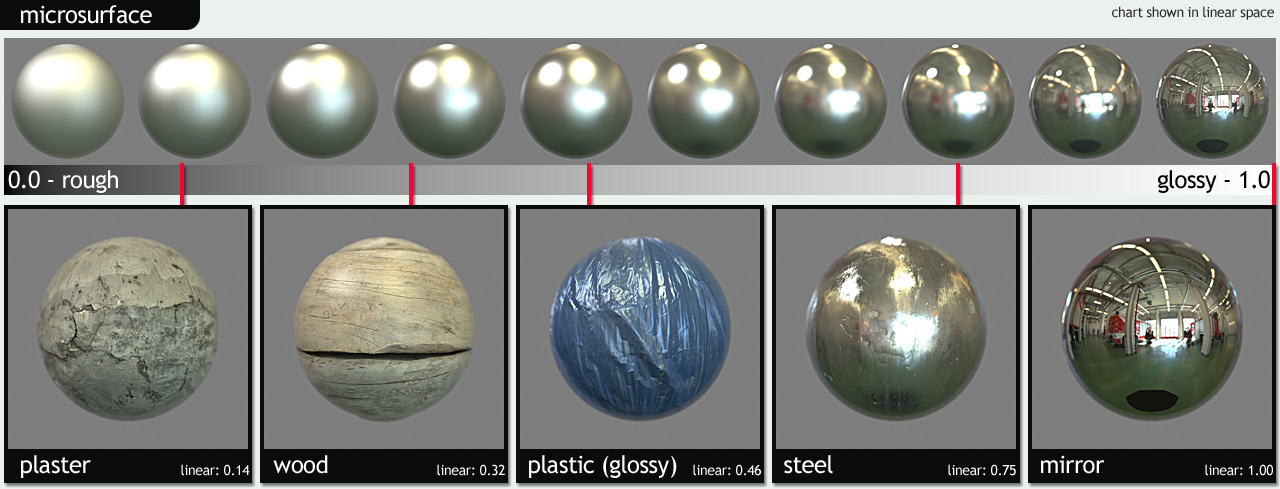
\includegraphics[width=13cm]{microcompare05.jpg}
            %     \caption[Project Schedule] {
            %         Generated spheres using Physically Based Rendering \citep{pbr}.
            %     }
            %     \label{figure:pba}
            % \end{figure}

            % Images of balls that are primarily metallic or
            % transparent will also not be included in the initial dataset. To begin with, the images
            % should contain an individual ball or disk and then progress to
            % having both, or a combination of, within the same image. This will
            % test whether our methods of detection are able to identify
            % multiple spheres correctly. Some images may feature:

            % \begin{itemize}
            %     \item Objects that appear as spheres from different angles.
            %     \item Non-spherical objects.
            %     \item An aspheric (deflated) sphere.
            %     \item Spheres that intersect with each other.
            %     \item Disks that intersect with each other.
            %     \item A sphere and disk that intersect with each other.
            %     \item A sphere or disk that is rotated. \todo{what is rotated and why}
            %     \item A sphere or disk that is partially cropped out.
            % \end{itemize}

            % It is of significant importance to create a dataset that features an
            % array of environments, to ensure that the sphere detection methods are
            % robust and able to function in as many scenarios as possible. These
            % environments have been grouped into four distinct categories:

            % \begin{enumerate}
            %     \item \textbf{Soccer:} This is a standard indoor robot soccer
            %     environment.
            %     \item \textbf{Uniform:} The environment is plain and largely the same
            %     colour.
            %     \item \textbf{Textured:} The environment contains textures and
            %     repeatable patterns.
            %     \item \textbf{Cluttered:} The environment contains many objects that
            %     may obscure the detection of spheres.
            % \end{enumerate}

            % And may exhibit the following range of lighting conditions:

            % \begin{itemize}
            %     \item The number of lights vary.
            %     \item The position of the lights vary.
            %     \item The scene is lit from a single light source.
            %     \item The scene is lit from multiple light sources in a similar direction.
            %     \item The scene is lit from multiple light sources from different directions.
            %     \item The lighting is under normal conditions.
            %     \item The lighting is dim.
            %     \begin{itemize}
            %         \item The shadow of the ball should blend with the environment.
            %     \end{itemize}
            %     \item The lighting is bright.
            %     \begin{itemize}
            %         \item The lighting of the ball should blend with the environment.
            %     \end{itemize}
            % \end{itemize}

            % The dataset should also include a good combination of features and
            % environment configurations to test more complex cases. For example, two
            % intersecting spheres of the same colour under dim lighting will be far
            % more difficult to identify than two individual spheres of differing
            % colours in good lighting. The texture of the sphere should also be
            % considered as it can effect the type of lighting that is emitted.

            % The positions and sizes of the spheres within the dataset will be
            % specified by drawing boxes around them, so these cropped images can be
            % used to train the classifiers.

        }

    }

    \section{Preliminary Results} {
    \label{sec:results}

        The development portion of our project is only partially complete, as outlined in Section~\ref{sec:schedule}, but enough work has been completed to produce some preliminary results.

        A subset of the proposed image database has been obtained based on the ImageNet synset IDs listed in Table~\ref{tab:imagenet} for the positive images. A large collection of images from another source were used as negative images. Negative images for the final report will be sourced from ImageNet.

        Several Haar cascade classifiers were trained on this datset, using different training parameters, and their performances compared qualatitively by viewing the claissifier output on a small set of test images.

        The preliminary results obtained are summarised in Table~\ref{table:interim-results}.
        These results show that the resulting quality of a classifier is extremely sensitive to the training data and settings used.
        Some of the classifiers trained show promise, in that they detect balls in some of the images, and appear to detect circular objects in others, but it is clear that most of the supposed detections are false positives.
        The authors suspect that there are two main reasons for the low classification performance:

        \begin{itemize}
            \item The set of positive examples is too small and too varied; and
            \item The set of negative examples is poor, in that the images it contains are far too dissimilar from spheres.
                  The use of different ImageNet synsets, such as `n03032811 - Circle, round' into the set of negative samples may improve performance, and will be considered before the final report.
        \end{itemize}

        The remainder of the project shall have to focus on improving the training data and training method if a reliable sphere detector is to result, especially if it is to acheive our goal of distinguishing spheres and disks.

        \begin{table}[H]
            \caption{Summary of preliminary results. The important configuration parameters of each classifier are shown, along with several sample images indicating classification performance.}
            \centering
            % \resizebox{\linewidth}{!}{\begin{tabularx}
{\textwidth}{llllll}
    \toprule
    \textbf{Image dimensions} & \textbf{\# pos. samples} & \textbf{\# neg. samples} & \textbf{\# stages} & \textbf{Training time} & \textbf{Results} \\
    \midrule
    5x5 & 5 & 10 & 20 & 5 hours & sdfsdf \\
    \bottomrule
\end{tabularx}}
            \makebox[\textwidth][c]{\resizebox{0.5\paperwidth}{!}{\begin{tabularx}
{\textwidth}{llllll}
    \toprule
    \textbf{Image dimensions} & \textbf{\# pos. samples} & \textbf{\# neg. samples} & \textbf{\# stages} & \textbf{Training time} & \textbf{Results} \\
    \midrule
    5x5 & 5 & 10 & 20 & 5 hours & sdfsdf \\
    \bottomrule
\end{tabularx}}}
        \end{table}

    }

    \section{Project schedule} {
    \label{sec:schedule}

        The project plan outlined in Section~\ref{sec:plan} is to be achieved
        according to the schedule presented in the Gantt chart in
        Figure~\ref{gantt:proposal}.

        In response to the preliminary results in Section~\ref{sec:results}, the
        remainder of the project will focus on curating the image database,
        and tuning the training parameters of the classifiers to optimise the
        resulting classifier performance. This process will be iterated, using
        progressively larger datasets, until an approach for training a
        successful classifier on a large dataset is found. Once successful
        training methods are found for each type of classifier, several days
        will be dedicated to running the classifier training. The trained
        classifiers will be compared on a test set, and the results summarised
        in a report. If training of classifiers is found to be sufficiently
        fast, ROC curves will be generated for each of the feature types, and
        included in the report.

        \begin{figure}[H]
            \makebox[\textwidth][c]{\resizebox{0.95\paperwidth}{!}{% Define some Gantt chart helper commands:
\newcommand{\completedganttbar}[4][]{ %
    \ganttbar[bar/.append style={draw=gray, fill=gray},#1]{#2}{#3}{#4} %
}
\newcommand{\optionalganttbar}[4][]{ %
    \ganttbar[bar/.append style={draw=gray, pattern color=gray, pattern=north west lines},#1]{#2}{#3}{#4} %
}
\newcommand{\optionalganttlinkedbar}[4][]{ %
    \ganttlinkedbar[bar/.append style={draw=gray, pattern color=gray, pattern=north west lines},#1]{#2}{#3}{#4} %
}

\begin{ganttchart}[
        hgrid,
        vgrid={*6{black, dotted},*1{black, dashed}}, % Note: NO SPACES!
        title height = 1,
        x unit=0.3cm,
        y unit title=0.75cm,
        y unit chart=1cm,
        time slot format=isodate,
        % progress=today,
        % today=2015-8-20,
        % bar/.append style={fill=green},
        % bar incomplete/.append style={fill=white},
        % group incomplete/.append style={draw=black,fill=none},
        % progress label text={}
        ]
        {2015-03-16} % start date: Mon, Mar-16. Week 4.
        {2015-05-31} % end date: Sun, May-31.
\setganttlinklabel{f-s}{}

% Gantt chart header:
% Note: Week starts on Sunday.
\gantttitlecalendar*{2015-03-16}{2015-05-31}{month=name} \\
\gantttitlecalendar*{2015-03-16}{2015-04-05}{week=4}
\gantttitle{Semester 1 Recess}{14}
\gantttitlecalendar*{2015-04-20}{2015-05-31}{week=7}

% Proposal
\ganttnewline \ganttgroup{Project proposal}{2015-03-19}{2015-03-26}
\ganttnewline \ganttbar{Proposal preparation}{2015-03-19}{2015-03-23}
\ganttnewline \ganttbar{Presentation}{2015-03-24}{2015-03-26}

% Project work
\ganttnewline \ganttgroup{Project work}{2015-03-27}{2015-04-30}
\ganttnewline \ganttbar{Dataset collection}{2015-03-27}{2015-04-05}
\ganttnewline \ganttbar{Candidate selection}{2015-04-01}{2015-04-08}
\ganttnewline \ganttbar{Development}{2015-04-09}{2015-05-21}
\ganttnewline \ganttbar{Draft report preparation}{2015-04-23}{2015-04-30}

% Final report
\ganttnewline \ganttgroup{Final report}{2015-04-31}{2015-05-28}
\ganttnewline \ganttbar{Detection performance testing}{2015-04-31}{2015-05-21}
\ganttnewline \ganttbar{Analysis of results}{2015-05-08}{2015-05-28}
\ganttnewline \ganttbar{Final report preparation}{2015-05-16}{2015-05-28}

% % Examples of gantt chart capabilities: 
% \ganttnewline \ganttgroup{Label Text}{2015-08-20}{2015-10-5}
% \ganttnewline \ganttmilestone{Label Text}{2015-08-3}
% \ganttnewline \completedganttbar{Label Text}{2015-8-9}{2015-8-13}
% \ganttnewline \ganttlinkedmilestone{Label Text}{2015-08-19}
% \ganttnewline \ganttbar{Label Text}{2015-09-11}{2015-10-5}
% \ganttnewline \optionalganttbar{Label Text}{2015-10-6}{2015-10-26}

\end{ganttchart}
}}
            \caption[Project Schedule] {
                A Gantt chart illustrating the planned project schedule.
                Solid grey bars represent completed tasks.
            }
            \label{gantt:proposal}
        \end{figure}
    }

    \section{Roles and responsibilities} {

        Given the small size of the team, it will be easier to distribute the workload evenly if no particularly role is assigned to an individual. This means each researcher will equally contribute to the research, development and documentation of the project. Each researcher is committed to spending on average 8 hours of work per week to ensure that the project is completed on schedule.

        Researchers will seek academic advice from their supervisors and colleagues if and when necessary.
    }

    \section{Communication of results} {

        The results of the project will be compiled into a report, as outlined
        in the project schedule, that is intended to be suitable for
        submission to a relevant conference or journal. In the case that the
        report is accepted for publication, the dataset created for the
        project will also be made available online, along with the associated code.

    }

    \bibliography{bibliography}
    \bibliographystyle{apalike}

\end{document}

